\newpage

\anonchapter{Лабораторная работа №3}
\setcounter{chapter}{3}
\setcounter{section}{0}
\setcounter{figure}{0}
\setcounter{table}{0}
\setcounter{equation}{0}

\begin{center}
Определение подвижности основных носителей заряда \\
(4 часа)
\end{center}

\section{Цель работы}
Определение подвижности основных носителей заряда в полупроводнике и коэффициента Холла по измерениям эффекта холла.

\section{Теоретическая часть}

\subsection{Возникновение поля Холла}

Эффект Холла заключается в возникновении поперечного электрического поля в образце, через который протекает электрический ток, помещённом в магнитное поле, перпендикулярное направлению этого тока. Если в магнитном поле с индукцией $\overrightarrow{B}$ находится полупроводник n-типа, по которому течёт ток плотностью $\overrightarrow{j}$, то на электроны, движущиеся со скоростью $\overrightarrow{v}$ будет действовать сила Лоренца, отклоняющая их в сторону. Таким образом, на одной из граней появится отрицательный заряд, а на другом начнут скапливаться нескомпенсированные доноры. В дырочном полупроводнике механизм останется тем же, но знаки зарядов и направление их движения изменятся (см. рисунок \ref{pic3_lorentz}).

\begin{figure}[h!]\centering
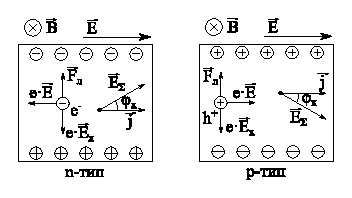
\includegraphics[height=4cm]{pic3_lorentz.eps}
\caption{Проявление эффекта Холла в образцах n- и p-типа проводимости.}
\label{pic3_lorentz}
\end{figure}

Возникающие на гранях, параллельных течению тока и индукции магнитного поля, заряды, создают электрическое поле $\overrightarrow{E}_{\text{х}}$, стремящееся компенсировать отклонение зарядов под действием силы Лоренца. Суммарное поле $\overrightarrow{E}_{\Sigma}$ будет направлено под углом $\phi$ к току, направление которого не изменится. Напряжённость поля $\overrightarrow{E}_{\text{х}}$ пропорциональна векторному произведению $\overrightarrow{B}$ и $\overrightarrow{j}$ с коэффициентом пропорциональности $R_{\text{х}}$.

\begin{equation}
\overrightarrow{E}_{\text{х}} = \overrightarrow{R}_{\text{х}} \left[ \overrightarrow{B} \times \overrightarrow{j} \right]
\label{eq3_vector_lorentz}
\end{equation}

$R_{\text{х}}$ называется коэффииентом Холла, а $\phi$ - углом Холла.

Как видно из рисунка \ref{pic3_lorentz}, направление силы Лоренца не зависит от знака заряда, а значит по направлению поля Холла можно определить тип основных носителей заряда в полупроводнике. Коэффициент Холла отрицателен в полупроводнике n-типа, и положителен для p-типа.

\subsection{Определение коэффициента Холла}

Если все углы между $\overrightarrow{B}$, $\overrightarrow{j}$ и $\overrightarrow{E}_{\text{х}}$ прямые, и не учитывается распределение электронов по скоростям, то (\ref{eq3_vector_lorentz}) можно переписать как

\begin{equation}
E^{y}_{\text{х}} = \frac{1}{e n} j^{x} B^{z}
\end{equation}
где $e$ - заряд электрона, $n$ - концентрация свободных носителей заряда.

В таком случае $R_{\text{х}} = \frac{1}{e n}$. Для учёта различия между полной скоростью электронов, входящей в выражение для силы Лоренца, и дрейфовой скоростью, которую электрон принимает под действием поля, а также распределения электронов по скоростям, решается кинетическое уравнение Больцмана. Точное решение приводит к необходимости введения коэффициента $r_{\text{х}} = \frac{<\tau^{2}>}{<\tau>^2}$, называемого холл-фактором, $\tau$ - время релаксации при данном основном механизме рассеяния.. В таком случае полное выражение для коэффициента Холла выглядит следующим образом:

\begin{equation}
R_{\text{х}} = \frac{r_{\text{х}}}{e n}
\end{equation}

Расчёты показывают, что для невырожденных полупроводников при рассеянии на акустических фононах $r_{\text{х}} = \frac{3}{8} \pi$, а при рассеянии на ионах примеси $r_{\text{х}} = \frac{315}{512} \pi$. Для вырожденных полупроводников и металлов величина $r_{\text{х}}$ от доминирующего механизма рассеяния не зависит и равна единице. Для сильных магнитных полей ($\mu B \gg 1$) коэффициент Холла не зависит от механизма рассеяния и степени вырождения, а определяется только концентрацией носителей заряда: $R_{\text{х}} = \frac{1}{e n}$.

В случае смешанной проводимости и в материалах близких к собственным коэффициент Холла опреедляется следующим соотношением:
\begin{equation}
R_{\text{х}} = \frac{r_{\text{х}}}{e} \frac{p \mu_{p}^{2} - n \mu_{n}^{2}}{\left( p \mu_{p} + n \mu_{n} \right)^{2}}
\end{equation}

В области примесной проводимости по коэффициенту Холла и электропроводности можно определить концентрацию основных носителей заряда, а по тангенсу угла Холла - их подвижность.

\subsection{Методика измерения и описание установки}

В ходе данной работы через образец, имеющий форму прямоугольного параллелепипеда, пропускается постоянный ток, и измеряется разность потенциалов, возникающая на холловских контактах (см. рисунок \ref{pic3_sample}). В данном случае

\begin{equation}
\begin{split}
V_{\text{х}} &= b E_{\text{х}} \\
V &= a E \\
I &= b d j
\end{split}
\end{equation}

\begin{figure}[h!]\centering
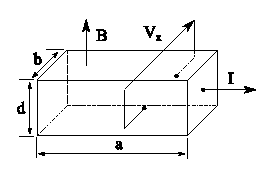
\includegraphics[height=4cm]{pic3_sample.eps}
\caption{Линейные размеры образца и расположение основных векторов}
\label{pic3_sample}
\end{figure}

Эти формулы можно переписать в виде:
\begin{equation}
\begin{split}
V_{\text{х}} &= - \frac{R_{\text{х}} I B}{d} \\
V &= \frac{I}{\sigma} \frac{c}{b d}
\end{split}
\end{equation}

Угол между направлением электрического поля в образце и полем Холла называется углом Холла и определяется как:
\begin{equation}
\tg \phi = \frac{E_{\text{х}}}{E} = \frac{a}{b} \frac{V_{\text{х}}}{V}
\label{eq3_tg}
\end{equation}

Измерив падение напряжения в продольном и поперечном направлении, а также индукцию магнитного поля, можно рассчитать основные характеристики образца:
\begin{equation}
\begin{split}
\sigma &= \frac{c}{b d} \frac{I}{V} \\
R_{\text{х}} &= d \frac{V_{\text{х}}}{I} \frac{1}{B} \\
\mu_{\text{х}} &= \frac{c}{b} \frac{V_{\text{х}}}{V} \frac{1}{B}
\end{split}
\label{eq3_mu}
\end{equation}

На точность измерения эффекта Холла влияет геометрия образца. Поперечное напряжение можно считать равным ЭДС Холла только при отношении длины образца к ширине не менее $3:1$.

Для измерения коэффициента Холла применяется стандартный метод постоянного тока и постоянного магнитного поля. Уменьшение вклада паразитных эффектов производится усреднением результатов измерения при разных направлениях тока и индукции. Пусть

\begin{equation}
\begin{split}
V_{I^{+}B^{+}} &= V_{\text{х}} + V_{\text{асм}} + V_{\text{мр}} + V_{\text{ТЭДС}} + V_{\text{Э}} + V_{\text{НЭ}} + V_{\text{ПНЭ}} + V_{\text{РЛ}} + V_{\text{ПРЛ}} \\
V_{I^{-}B^{+}} &= -V_{\text{х}} - V_{\text{асм}} - V_{\text{мр}} + V_{\text{ТЭДС}} - V_{\text{Э}} + V_{\text{НЭ}} - V_{\text{ПНЭ}} + V_{\text{РЛ}} - V_{\text{ПРЛ}} \\
V_{I^{-}B^{-}} &= V_{\text{х}} - V_{\text{асм}} - V_{\text{мр}} + V_{\text{ТЭДС}} + V_{\text{Э}} - V_{\text{НЭ}} + V_{\text{ПНЭ}} - V_{\text{РЛ}} + V_{\text{ПРЛ}} \\
V_{I^{+}B^{-}} &= -V_{\text{х}} + V_{\text{асм}} + V_{\text{мр}} + V_{\text{ТЭДС}} - V_{\text{Э}} - V_{\text{НЭ}} - V_{\text{ПНЭ}} - V_{\text{РЛ}} - V_{\text{ПРЛ}}
\end{split}
\end{equation}

$V_{\text{х}}$ - напряжение Холла.

$V_{\text{асм}}$ - напряжение асимметрии, возникающее, если холловские контакты находятся не на эквипотенциальных поверхностях. Знак не зависит от направления магнитного поля, но меняется вместе с направлением электрического поля.

$V_{\text{мр}}$ - магниторезистивный эффект, меняющий напряжение асимметрии. Знак зависит от направления тока.

$V_{\text{ТЭДС}}$ - термоэлектрический эффект, возникает между контактами при наличии градиента температур, одним из источников которого может быть неравномерность нагрева неоднородного образца. Зависит только от знака градиента температуры.

$V_{\text{Э}}$ - поперечный гальвано-термомагнитный эффект Эттинсгаузена, возникающий из-за наличия определённого распределения носителей по скоростям. Под действием магнитного поля быстрые горячие электроны отклоняются сильнее медленных холодных, из-за чего возникает поперечный градиеннт температур и связанная с ними термоЭДС. Знак зависит от направления тока, направления магнитного поля и знака носителей заряда.

$V_{\text{НЭ}}$ - поперечный термогальваномагнитный эффект Нернста-Эттинсгаузена, возникает из-за наличия продольного градиента температур. Энергия электронов, движущихся от горячего конца к холодному больше энергии в обратном потоке, эти потоки отклоняются в магнитном поле в разные стороны, возникает ток в поперечном направлении, который компенсируется током за счет ЭДС Нернста-Эттинсгаузена. Знак зависит от направления магнитного поля.

$V_{\text{ПНЭ}}$ - электротермически эффект Пельтье, приводящий к термогальваномагнитному эффекту Нернста-Эттинсгаузена, наблюдается если причиной возникновения грандиента температур является эффект Пельтье вблизи омических контактов. Знак зависит от направления тока и магнитного поля.

$V_{\text{РЛ}}$ - термомагнитный эффект Риги-Ледюка, поперечная термоЭДС, возникающая из-за продольного градиента температур. Знак зависит от направления магнитного поля.

$V_{\text{ПРЛ}}$ - эффект Пельтье, приводящий к возникновению продольного градиент температур и, как следствие, к термоЭДС Риги-Ледюка. Знак зависит от направления тока и направления магнитного поля.

Усреднённое напряжение на холовских контактах рассчитывается по формуле:
\begin{equation}
\overline{V}_{\text{х}} = \frac{V_{I^{+}B^{+}} - V_{I^{-}B^{+}} + V_{I^{-}B^{-}} - V_{I^{+}B^{-}}}{4} = V_{\text{х}} + V_{\text{Э}} + V_{\text{ПНЭ}} + V_{\text{ПРЛ}}
\end{equation}

Вкладом эффектов Пельтье-нернста-Эттинсгаузена и Пельтье-Риги-Ледюка во многих материалах, особенно высокоомных, можно пренебречь.

Если оборудование позволяет изменять только направление магнитного поля, среднюю величину рассчитывают по разности измеренных значений при разной полярности магнитного поля:

\begin{equation}
\overline{V}_{\text{х}} = \frac{V_{I^{+}B^{+}} - V_{I^{+}B^{-}}}{2} = V_{\text{х}} + V_{\text{Э}} + V_{\text{НЭ}} + V_{\text{ПНЭ}} + V_{\text{РЛ}} + V_{\text{ПРЛ}}
\end{equation}

В ходе работы через образец, помещённый между полюсами магнита, пропускается ток и снимается разность потенциалов между токовыми и холловскими выводами. Полученные данные считываются встроенными в лабораторный стенд АЦП и обрабатываются микроконтроллером, после чего передаются на компьютер. Значение магнитной индукции в диапазонах, используемых в данной работе, линейно зависит от тока через катушку. Блок-схема прибора приведена на рисунке \ref{pic3_scheme}. Все указанные на схеме вольтметры встроены в лабораторный стенд и отображаются в рабочей области программы. Приборы активируются щелчком мыши по соответствующему значку.

\begin{figure}[h!]\centering
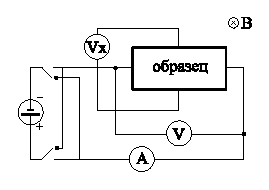
\includegraphics[height=4cm]{pic3_scheme.eps}
\caption{Линейные размеры образца и расположение основных векторов}
\label{pic3_scheme}
\end{figure}

\section{Порядок проведения работы и указания по технике безопасности}

\begin{enumerate}
\item Запустить прибор и программу для измерения эффекта Холла.
\item Выбрать схему измерения №1, активировать все блоки устройства.
\item Установить значение тока через образец равным 1 мА.
\item Провести серию измерений напряжения на образце $V$ и напряжения Холла $V_{\text{х}}$ изменяя индукцию магнитного поля от -150 до 150 мТл.
\item Повторить измерения при токе через образец равном 2 мА.
\end{enumerate}

Электрический ток в схеме не превышает 10 мА. При выполении работы действует стандартная техника безопасности при работе с компьютером.

\section{Обработка результатов эксперимента}

\begin{enumerate}
\item Результаты измерений занести в таблицу. Значения для положительных и отрицательных величин индукции магнитного поля вносятся в одну строку с указанием полярности.
\item Определить тангенс угла Холла из соотношения (\ref{eq3_tg}).
\item Определить тип и подвижность основных носителей заряда, пользуясь выражением (\ref{eq3_mu}).
\item Используя (\ref{eq3_mu}) найти коэффициент Холла, считая основным механизмом рассеяние на ионах примеси.
\item Определить погрешность измерения.
\end{enumerate}

\begin{table}[h!]
\caption{Измерение величины эффекта Холла}
\begin{center}
\begin{tabular}{c|c|c|c|c|c}
№ & I & $V_{B^{+}}$ & $V_{B^{-}}$ & $\overline{V}$ & $R_{\text{х}}$ \\
\hline
& мА & В & B & B & $\text{см}^{-3}\text{Кл}^{-1}$ \\
\hline
\end{tabular}
\end{center}
\end{table}

\section{Контрольные вопросы}

\begin{enumerate}
\item Каков механизм возникновения эффекта Холла?
\item Какие электрофизические свойства полупроводников можно исследовать с помощью эффекта Холла?
\item Как связаны коэффициенты Холла и концентрация носителей заряда в случае примесной и собственной проводимости?
\item Отклонение электронов и дырок под действием силы Лоренца.
\item Критерии слабых и сильных электрических и магнитных полей.
\item Дрейфовая и холловская подвижность свободных носителей заряда.
\item Определение Холл-фактора, его зависимость от степени вырождения и механизма рассеяния в полупроводнике.
\item Природа возникновения паразитных ЭДС, возникающих при исследовании эффекта Холла.
\item Как определить доминирующий механизм рассеяния носителей заряда?
\item Эффект Холла в полупроводнике со смешаным типом носителей заряда.
\end{enumerate}

\section{Литература}
\begin{enumerate}
\item П.С. Киреев. Физик полупроводников. М.: Высшая школа, 1975.
\item Шалимова К.В. Физика полупроводников. СПб.: Лань 2011. 416 с.
\item Абрамов В.Б., Аверин И.А., Карпанин О.В. и др. Исследование свойств полупроводников методом эффекта Холла. Методические указания. Пенза. ПГУ. 2010.
\end{enumerate}